\chapter{Technisches Konzept}
\label{cha:Technisches Konzept}

\section{Anforderungen an die Applikation}
\subsection{Nachrichtendarstellung und Filterung}
Ein zentraler Bestandteil der Applikation ist die nachträgliche Analyse von 
\acrshort{acr:MQTT}-Nachrichten. Im Gegensatz zu bestehenden Tools wie MQTT.fx soll die 
Anwendung die Möglichkeit bieten, bereits empfangene Nachrichten im 
Nachhinein zu filtern. Die Filterung erfolgt dabei auf Basis von 
Topic-Präfixen. Ergänzend dazu wird eine Volltextsuche benötigt, die eine 
schnelle Navigation innerhalb großer Datenmengen ermöglicht. Hierbei sollen 
sowohl die Payload, das Topic als auch der Zeitstempel durchsucht werden 
können. Ziel ist eine effiziente Analyse auch bei stark ansteigenden 
Nachrichtenvolumina.

Ein weiterer funktionaler Bestandteil ist die parallele Analyse mehrerer 
Datenströme. Hierzu soll die Applikation die gleichzeitige Anzeige mehrerer 
Log-Fenster ermöglichen. Für jedes dieser Fenster können individuelle Filter 
gesetzt sowie die dargestellten Inhalte separat exportiert werden. Dadurch 
wird eine flexible und unabhängige Auswertung verschiedener Topics 
ermöglicht.

\subsection{Automatische Fehlererkennung}
Die Anwendung soll darüber hinaus Funktionen zur automatischen 
Fehlererkennung bereitstellen. Dazu gehört die Validierung der Payloads auf 
korrektes JSON-Format sowie die Erkennung struktureller Abweichungen. Ein Beispiel für eine strukturelle Abweichung ist das Fehlen des sogenannten Headers im Payload, der in jeder Nachricht den Sender und weitere Nachrichtendetails wie den Nachrichtentyp beschreibt.
Zusätzlich sollen auch Fehler innerhalb von Maschinenprozessen anhand der Nachrichten erkannt werden. Dazu werden die beim Prozess versendeten Nachrichten mit vordefinierten erwarteten Nachrichten verglichen. Sollte hier eine Abweichung erkannt werden, soll die Anwendung eine entsprechende Fehlernachricht anzeigen. Ziel ist eine frühzeitige 
Identifikation fehlerhafter oder inkonsistenter Nachrichten. Ergänzend dazu 
muss eine Überwachung der Teilnehmer erfolgen, um festzustellen, ob alle Systemkomponenten mit dem Broker verbunden sind und ihre Verbindung aufrechterhalten.

\subsection{Überwachung der Automatisierungs-Abläufe}
In einem zusätzlichen Reiter sollen abgeschlossene und laufende Abläufe der Verpackungslinie eingesehen werden können. In den einzelnen Automatisierungs-Abläufen werden die erwarteten und bereits empfangenen Nachrichten dargestellt. Sollte ein neuer Prozess beginnen, während noch nicht alle erwarteten Nachrichten eingingen, wird der Prozess mit einer Fehlermeldung abgespeichert und angezeigt.

Zu den Abläufen gehören Linienstart und -stopp, Quittierung von Fehlermeldungen, Leerfahren der Linie, Artikelwechsel,  fliegender Artikelwechsel und Batchhandlingprozesse. Dabei können die Abläufe Fehlerquittierung, Linienstart und Linienstopp nicht parallel  laufen und allgemein kein Linienablauf gleichzeitig mehrfach aktiv sein. Dadurch können fehlerhaft abgeschlossene Abläufe erkannt werden.

\subsection{Simulationsmöglichkeiten}
Eine weitere Anforderung stellt die erweiterte Publish-Funktionalität dar. 
Nachrichten sind manuell erstellbar und können unter einem bestimmten Topic 
gesendet werden. Dabei ist vorgesehen, häufig genutzte Nachrichten 
als Vorlagen zu speichern und wiederzuverwenden. Zusätzlich soll die 
Möglichkeit bestehen, Nachrichten in festgelegten Zeitintervallen automatisch 
zu senden. Dies unterstützt insbesondere Test- und Simulationsszenarien.

Ergänzend dazu ist eine Simulationsfunktion vorgesehen, welche das Senden 
vordefinierter Nachrichten über eine direkte Benutzerinteraktion ermöglicht. 
Dabei soll die Initiierung solcher Aktionen durch konfigurierbare Bedienelemente erfolgen. Ziel ist eine vereinfachte Durchführung von Tests sowie der 
Erzeugung reproduzierbarer Datenströme.

\subsection{Anforderungen an die Performance}
Neben den funktionalen Anforderungen spielt die Performance der Anwendung eine 
entscheidende Rolle. Dies ist insbesondere bei hohen Nachrichtenfrequenzen in industriellen Anlagen relevant. Die Verarbeitung und Darstellung der Nachrichten muss so 
gestaltet sein, dass auch bei hohen Datenraten eine flüssige Bedienung 
gewährleistet bleibt. Gleichzeitig ist eine skalierbare Architektur notwendig, 
um zukünftige Erweiterungen des Funktionsumfangs zu ermöglichen.

Abschließend soll die Umsetzung dieser Anforderungen in einer übersichtlichen 
und intuitiv bedienbaren Benutzeroberfläche erfolgen. Auch bei komplexen 
Analyseprozessen muss eine schnelle Orientierung sowie eine effiziente 
Interaktion gewährleistet sein. Die übergeordnete Zielsetzung besteht darin, 
bestehende Werkzeuge in den Bereichen Datenanalyse, Fehlersuche und 
Testautomation funktional zu erweitern und insbesondere hinsichtlich 
Benutzerfreundlichkeit und Analysefähigkeit zu verbessern.

\subsection{Erweiterbarkeit und Zukunftssicherheit}
    Die Architektur soll so gestaltet werden, dass sie nicht nur für den aktuellen Zweck geeignet ist, sondern auch langfristig wartbar und erweiterbar bleibt. 
    Insbesondere in der Industrie und bei der Kommunikation mit \acrshort{acr:MQTT}-Systemen ändern sich die Anforderungen oft im Laufe der Zeit. Neue Maschinen, zusätzliche Linien, 
    neue Nachrichtentypen oder geänderte Datenstrukturen sind Beispiele dafür, auf die ein Überwachungstool flexibel reagieren muss.

    Ein wichtiger Aspekt der Erweiterbarkeit besteht darin, fachliche Regeln und Prüfmechanismen nicht direkt im Programmcode zu verankern, 
    sondern sie über Konfigurationsdateien abzubilden. In diesem Konzept wird dies durch den Einsatz externer JSON-Dateien umgesetzt. Sowohl die Teilnehmerüberprüfung 
    als auch die optionale Schema-Validierung sollen auf Konfigurationsdateien basieren, die zur Laufzeit geladen werden können. Dadurch können neue Teilnehmer, Maschinen oder 
    Validierungsregeln hinzugefügt werden, ohne dass die Applikation angepasst oder neu kompiliert werden muss.

    Die optionale Schema-Validierung ist ein wichtiger Baustein für die Zukunftssicherheit. Durch die Nutzung versionierter Nachrichtenschemas können verschiedene 
    Nachrichtenformate parallel unterstützt werden. In realen Produktionsumgebungen ist es selten der Fall, dass alle Systeme gleichzeitig auf eine neue Software- 
    oder Protokollversion aktualisiert werden. Die Fähigkeit, mehrere Schema-Versionen zu erkennen und zu validieren, ermöglicht einen schrittweisen Übergang zwischen 
    verschiedenen Versionsständen. Alte Systeme bleiben weiterhin analysierbar, während neue Systeme bereits mit erweiterten oder geänderten Datenstrukturen arbeiten können.

    Ein weiterer wichtiger Faktor für die Erweiterbarkeit ist die lose Kopplung der einzelnen Schichten. Die Netzwerkschicht ist ausschließlich für die \acrshort{acr:MQTT}-Kommunikation zuständig und hat kein Wissen über die interne Darstellung oder die Analyseergebnisse der Nachrichten. Ebenso ist die grafische Oberfläche von der konkreten Netzwerktechnik entkoppelt und arbeitet ausschließlich mit Datenmodellen und Analyseergebnissen. Diese Trennung ermöglicht es, einzelne Komponenten auszutauschen oder zu erweitern, ohne unbeabsichtigte Auswirkungen auf andere Teile der Applikation zu verursachen. Diese lose Kopplung wird durch die Verwendung von Interfaces sowie klar definierten Service-Schichten umgesetzt.

    Auch die Analyse- und Validierungslogik soll bewusst modular aufgebaut werden. Die mehrstufige Verarbeitung ermöglicht es, zusätzliche Prüfungen schrittweise zu ergänzen. 
    Neben den bereits vorgesehenen Basis- und Konsistenzprüfungen können zukünftig weitere Analysearten integriert werden. Denkbar sind beispielsweise zeitbasierte Prüfungen, 
    bei denen Nachrichten auf erwartete Wiederholungsintervalle oder Heartbeat-Mechanismen überprüft werden.

    Die Nutzung eines datengetriebenen GUI-Konzepts trägt ebenfalls wesentlich zur Zukunftssicherheit bei. Da die Benutzeroberfläche nicht direkt durch Programmcode 
    manipuliert wird, sondern sich automatisch aus den zugrunde liegenden Datenmodellen aktualisiert, kann das grafische Erscheinungsbild flexibel erweitert werden. 
    Neue Ansichten, Filterfunktionen oder Darstellungsformen lassen sich hinzufügen, ohne die zugrundeliegende Analyse-Logik anpassen zu müssen.

    Ein weiterer Aspekt der Zukunftssicherheit ist die Skalierbarkeit hinsichtlich der Nachrichtenlast. Ein zentraler Bestandteil ist dabei die Nutzung von asynchronen Programmiertechniken (async/await), die eine nicht-blockierende Verarbeitung von Nachrichten ermöglicht. 

    Abschließend lässt sich festhalten, dass die konzipierte Architektur bewusst auf langfristige Nutzung und Erweiterbarkeit ausgelegt sein soll. 
    Durch konfigurationsgetriebene Validierungsmechanismen, versionierte Nachrichtenschemas, lose Kopplung der Systembestandteile sowie eine datengetriebene Benutzeroberfläche soll eine hohe Flexibilität erreicht werden. Diese Eigenschaften machen das Überwachungstool nicht nur für den aktuellen Entwicklungsstand praktikabel, sondern erlauben auch eine zukünftige Anpassung an neue Anforderungen, ohne eine grundlegende Neugestaltung der Applikation erfordern zu müssen. Neben diesen Vorteilen bringt diese Anforderung einen wesentlich erhöhten Programmieraufwand mit sich, der in einer Projektarbeit teilweise nicht umsetzbar sein kann. 

\section{Prototypische Umsetzung und Erkenntnisse aus der Entwicklung}
    \subsection{Umsetzung des Prototyps in Python}
        Zum Testen der Realisierbarkeit der Applikation und ihrer Anforderungen wird ein Prototyp eines ersten funktionalen Systems zur Überwachung von \acrshort{acr:MQTT}-Nachrichten entwickelt. Dabei liegt der Fokus zunächst auf dem Empfang und der Darstellung der Nachrichten, der Analyse ihrer Inhalte sowie der damit verbundenen Erkennung einfacher Fehler. Die Umsetzung ist bewusst minimal gehalten, um nur Grundfunktionalitäten zu testen.

        Für die prototypische Umsetzung wird Python in Kombination mit dem GUI-Framework Tkinter verwendet. Dieses Framework gilt als sehr leichtgewichtig und vereinfacht die Erstellung des \acrshort{acr:GUI} stark \autocite{TkinterPythonInterface}. Bereits der Prototyp weist einen modularen Aufbau auf, indem das Programm in mehrere, nach Aufgaben gegliederte Dateien aufgeteilt ist. 

        Für die Architektur des Prototyps existiert eine zentrale Klasse \enquote{MQTTGui}. Diese ist für die Erstellung der grafischen Oberfläche, aber auch für die Datenhaltung über die Arrays "self.messages" und "self.topics" zuständig. Die \acrshort{acr:GUI} besteht aus einer Log-Anzeige, Fehleranalyse und der Verbindungssteuerung. 

        \subsection{Verbindungsaufbau und Nachrichtenempfang}
        Der Verbindungsaufbau wird in der Subscriber-Klasse implementiert. Dazu wird ein Objekt der Klasse \textit{MQTT\_Subscriber} erstellt und diesem die in der \acrshort{acr:GUI} eingegebenen Broker-IP und Port übergeben. Dadurch verbindet sich das Programm mit dem Broker und abonniert alle Topics. Bei der Erstellung des Objekts wird auch eine Callbackfunktion übergeben, die immer aufgerufen wird, wenn neue Nachrichten eintreffen (Listing: \ref{lst:Message-Empfang}). 

        \begin{lstlisting}[
        language=Python,
        caption={Callbackfunktion für den Message-Empfang},
        label={lst:Message-Empfang}
        ]
def on_message(self, topic, payload, qos, retained):
    ts = datetime.now().strftime("%Y-%m-%d %H:%M:%S")
    self.messages.append((ts, retained, topic, payload, qos))

    self.tool_pane.analyze_messages(self.messages, only_new=True)

    if self.save_var.get():
        log_to_file(topic, payload, qos, retained)
        \end{lstlisting}

        In dieser Callback-Funktion wird jede Nachricht in \enquote{self.messages} mit Zeitstempel, dem Topic, Payload und dem \acrshort{acr:QoS} gespeichert und an die Fehleranalyse-Komponente übergeben. Optional können die Nachrichten auch in einer externen Datei gespeichert werden.

    \subsection{Nachrichtenverarbeitung}
        Die Darstellung der Nachrichten in einem oder in verschiedenen Nachrichtenfenster implementiert die Klasse \enquote{LogPane}. In dieser wird neben Autoscroll-Funktionen auch eine Filterung nach Topics erstellt, die man in der \acrshort{acr:GUI} für jedes Nachrichtenfenster einzeln anwenden kann. Damit nur die Nachrichten der einzelnen Topics angezeigt werden, wird in der Methode \textit{append} herausgelesen, was in dem Filter eingegeben ist, und entscheidet auf dieser Grundlage über das Einfügen der einzelnen Nachrichten in die jeweilige Nachrichtenliste (Listing: \ref{lst:filtered_display}).
        \begin{lstlisting}[
        language=Python, 
        caption={gefilterte Anzeige von Nachrichten},
        label={lst:filtered_display}
        ]
def append(self):
    f = self.filter.get()
    for ts, retained, topic, payload, qos in self.messages[self.last_index:]:
        if f == "ALL" or topic.startswith(f):
            self._insert(ts, retained, topic, payload, qos)
    self.last_index = len(self.messages)
        \end{lstlisting}

    \subsection{Umgang mit großen Datenmengen}
        Als weitere Funktion werden sehr große Payloads, die für die Anzeige die \acrshort{acr:GUI} stark belasten, ausgelagert. Durch einen Klick auf die Nachricht wird diese in einem externen Editor geöffnet. Ähnlich funktioniert auch das Aufrufen der Nachricht durch das Anklicken der Fehlermeldung in der Analysekomponente. In diesen Fehlermeldungen werden jeweils die Nachrichten- sowie Fehlernummern gespeichert. Beim Anzeigen der Fehlermeldung wird der Nachricht ein sogenannter \textit{Tag} übergeben. Dieser enthält die Fehlernummer und die Methode, die abgearbeitet werden soll, wenn auf die Nachricht geklickt wird. In diesem Fall wird die Methode \textit{on\_error\_click} aufgerufen (Listing: \ref{lst:error-click}).
        \begin{lstlisting}[
        language=Python, 
        caption={gefilterte Anzaige von Nachrichten},
        label={lst:error-click}
        ]
def on_error_click(self, index):
    if not self.logpane:
        return
    self.gui.show_logs()
    error = self.errors[index]
    msg_id = error.get("msg_id")
    if msg_id is None:
        return
    
    self.logpane.jump_to_message(msg_id)
        \end{lstlisting}

        Für die fertige Applikation darf eine sehr große Datenmenge kein Problem darstellen. Deswegen ist es wichtig, dass von Anfang an großen Wert auf die Performance und Stabilität des Programms gelegt wird. 

        Durch die Implementierung einer separaten Analysekomponente können die Nachrichten auf das Vorhandensein eines Topics und Payloads überprüft werden. Des Weiteren werden die Payloads daraufhin auf ein korrektes JSON-Format überprüft. Als Zusatzfunktion dieser Analysekomponente kann eine sogenannte \textit{Line-Config}-Datei aus den Dateien heraus geladen werden. Diese beinhaltet alle Teilnehmer mit (Host-)Namen im JSON-Format. So kann überprüft werden, ob sich alle Teilnehmer beim Broker registrierten und auch weiterhin die Verbindung zum Broker nicht wieder schließen.

        Somit enthält bereits der Prototyp einige Anforderungen an die Applikation und kann bereits für einfache Analysen eingesetzt werden. 
    \subsection{Grenzen des Prototyps}
        Im Rahmen der prototypischen Umsetzung mit der verwendeten Struktur wurden klare Grenzen identifiziert. Insbesondere die grafische Darstellung in Python kommt bei zunehmender Komplexität an ihre Grenzen.
        Vor allem umfangreiche Datenbindung, visuell komplexe Tabellenansichten oder eine tiefe Integration mit dem Betriebssystem lassen sich in dem Python-GUI-Framework nur begrenzt
        elegant umsetzen. Erweiterungen oder individuelle Anpassungen führen oft zu hohem Implementierungsaufwand und schlechter Wartbarkeit. Dies ist jedoch nicht ausschließlich auf die Programmiersprache Python zurückzuführen, sondern liegt auch an der geringen Modularisierung und Performance-Auslegung des Programms und ist teilweise auf die gewählte Architektur zurückzuführen. Dadurch wird aber deutlich, dass für die Programmierung in C\# von Anfang an stark modularisiert werden muss, damit das Programm langfristig erweiterbar und leicht anpassbar bleibt. Des Weiteren muss in C\# eine asynchrone Performance-orientierte Verarbeitung der Nachrichten  ermöglicht werden, damit diese die UI nicht blockieren und das Programm aufgrund von zu großen Datenmengen abstürzt.

        Die interpretierte Programmiersprache Python weist im Vergleich zu kompilierten Sprachen wie C\# eine geringere Laufzeitperformance auf \autocite{PythonVSCS}. Besonders bei hohen Nachrichtenraten oder großen Datenmengen kann es zu Verzögerungen in der Verarbeitung und Darstellung kommen. Dies spielt gerade bei der Speicherung der Nachrichten in externe Text-Dateien oder Datenbanken eine große Rolle, da dieser Vorgang mehr Zeit beansprucht.  Für solche Prozesse bietet Python dafür die Bibliothek ,,asyncio'', mit der asynchrone Prozesse effizient verwaltet und ereignisgesteuert ausgeführt werden können. Diese wurde jedoch in dem Prototyp nicht verwendet, weswegen die Performance verschlechtert wird \autocite{AsyncioAsynchronous}.

        Für eine produktive Anwendung bestehen jedoch klare Anforderungen an Performance, Wartbarkeit, Typensicherheit und Integration. Diese Anforderungen sprechen deutlich für eine Neuimplementierung in C\#. Diese Programmiersprache bietet eine bessere Unterstützung für asynchrone Verarbeitungen, moderne \acrshort{acr:GUI}-Frameworks wie \acrshort{acr:WPF} und ermöglicht eine stärkere Integration in Windows-Systeme \autocite{PythonVSCS}. Dadurch wird eine langfristig stabile, erweiterbare und performante Lösung ermöglicht. 

        Die gewonnenen Erkenntnisse aus dem Prototypen fließen direkt in die Konzeption der finalen Applikation ein. 

   \section{Konzeptplan und Umsetzung der Benutzeroberfläche}

\subsection{Systemarchitektur}
Als Architekturgrundstein für die Applikation wird die \acrshort{acr:MVVM} (\acrlong{acr:MVVM})-Architektur genutzt. Durch diese Architektur entsteht eine saubere Trennung von UI und Logik. Die View dient dabei ausschließlich der Darstellung, während das View-Model die Logik
 und Bereitstellung der Daten für das View beinhaltet. Im UI-Programmcode selbst existiert dabei bestenfalls keinerlei Logik. Die Bereitstellung der Daten erfolgt durch die Models.

Durch dieses Modell entsteht wenig Code für die UI, da diese lediglich sogenannte Bindings hinterlegt, die von den View-Models gesteuert werden. So können die View-Models und Models auch ohne UI getestet werden und die View jederzeit einfacher ersetzt werden. 

In diesem Projekt werden die View-Models durch Service- und Repository-Dateien unterstützt, in denen die Anwendungslogik verankert ist. Dadurch übernimmt das View-Model ausschließlich die Interaktion mit der Benutzeroberfläche und die Bereitstellung der Daten. Die Repository-Dateien übernehmen die Aufgabe der Initialisierung der Tabellen in der Datenbank
 sowie Speicherung und Laden von Daten aus der Datenbank. Die Service-Dateien verarbeiten die Daten der View-Models und rufen wenn nötig die Methoden der Repositorien auf.

Die Verbindung zwischen View und View-Model erfolgt über das Data-Binding-System von WPF. Dabei wird dem \lstinline|DataContext| einer View ein entsprechendes ViewModel zugewiesen. Die Benutzeroberfläche kann anschließend über Bindings auf die Eigenschaften und Befehle des View-Models zugreifen, ohne dieses direkt zu kennen. Dadurch entsteht eine lose Kopplung zwischen Darstellung und Anwendungslogik \autocite{michaelstonisModelViewViewModelNET}.

Änderungen an Eigenschaften des View-Models werden über das Interface \lstinline|INotifyPropertyChanged| an die View weitergegeben. Dadurch werden zum einen Änderungen aus der View automatisch in die Variablen der View-Model geschrieben, zum anderen Änderungen aus dem View-Model automatisch in der Benutzeroberfläche dargestellt. Für Auflistungen wird eine \lstinline|ObservableCollection| verwendet, die Änderungen innerhalb einer Sammlung selbständig an die View weitergibt. Benutzerinteraktionen wie beispielsweise das Betätigen eines Buttons oder die Auswahl eines Tabelleneintrags können über Commands an das View-Model weitergeleitet werden. Die eigentliche Verarbeitungslogik verbleibt dabei im View-Model, während die View ausschließlich für die Darstellung und Entgegennahme von Benutzereingaben zuständig ist \autocite{michaelstonisModelViewViewModelNET}.

Zur erleichterten Umsetzung der MVVM-Struktur wird die ,,CommunityToolkit.Mvvm''-Bibliothek verwendet. Mit dieser Bibliothek kann zum einen die ansonsten aufwendige Implementierung des Interfaces \lstinline |INotifyPropertyChanged| erleichtert werden. Mittels Source-Generatoren wird die benötigte Property-Changed-Logik automatisch erzeugt. Dadurch kann redundanter Boilerplate-Code vermieden werden, was sowohl den Implementierungsaufwand als auch die Lesbarkeit des Quellcodes verbessert \autocite[S. 106 ff.]{nijsMVVMPatternNET2023a}.

Darüber hinaus ermöglicht die Bibliothek CommunityToolkit.Mvvm eine einfache Implementierung von \lstinline|ICommand|-Schnittstellen. Diese werden benötigt, um Benutzerinteraktionen wie beispielsweise Button-Klicks an das ViewModel weiterzuleiten. Während ohne die Bibliothek zusätzlicher Programmieraufwand für die Implementierung eines Commands erforderlich ist, genügt mit CommunityToolkit.Mvvm die Verwendung des Attributs \lstinline|[RelayCommand]| oberhalb der entsprechenden Methode. Aus dieser Methode wird automatisch ein Command erzeugt, welches anschließend über ein Binding in der View verwendet werden kann \autocite[S. 106 ff.]{nijsMVVMPatternNET2023a}.
\subsection{Datenbankkonzept}
Ziel des Datenbank-Designs ist die Speicherung aller MQTT-Nachrichten, eine effiziente Suche in allen Nachrichten, die Teilnehmer und Statusüberwachung, eine Prozessanalyse und die Speicherung von Vorlagen und Einstellungen.
Dazu werden unterschiedliche Haupttabellen erstellt.

Die Tabelle \textit{Messages} speichert die ID, Zeitstempel, Topic, Payload und den Sender der Nachricht. Die Tabelle \textit{Participants} speichert die Namen und den Maschinentyp aller Teilnehmer sowie deren zuletzt gesehener Zeitstempel, den Status und den Zustand, in dem sie sich gerade befinden.
In der Tabelle \textit{Errors} werden alle Fehler mit der entsprechenden Nachrichten-ID sowie Fehlertext und -Art gespeichert.
In der Tabelle \textit{ProcessEvent} werden die verschiedenen durchlaufenen Prozesse sowie deren Startzeit, Endzeit, bereits empfangene Nachrichten und die als Nächstes erwarteten Nachrichten gespeichert.

Die bereits beschriebenen Tabellen sollen ihren Inhalt beim Starten der Anwendung und bei der manuellen Verbindungstrennung zum Broker wieder löschen, damit die Nachrichten, Teilnehmer und Prozesse bei einer neuen Verpackungslinie auch wieder neu aufgezeichnet werden können. Die folgenden Tabellen besitzen dieses Verhalten gezielt nicht, da diese Informationen zwischen verschiedenen Anwendungssitzungen gespeichert werden sollen.

In den Tabellen \textit{TemplatesConnection} und \textit{TemplatesPublishingMessages} werden Vorlagen für Verbindungen sowie für zu versendende Nachrichten gespeichert. Dadurch können gespeicherte Vorlagen per Mausklick für den Verbindungsaufbau oder das Senden von Nachrichten verwendet werden.
In Settings werden alle Einstellungen gespeichert, damit diese auch bei einem Neustart der Anwendung noch gespeichert sind.

\subsection{Nachrichtenfluss und -Verarbeitung}
Beim Eintreffen einer Nachricht soll eine Callback-Funktion über ein Event aufgerufen werden. Diese übernimmt dann zum einen die Aktualisierung der UI, ruft zum anderen aber auch einen Service auf, der sich der Verarbeitung der Nachricht widmet. 
In Abbildung \ref{fig:FloatchartMessages} ist der Ablauf für diesen Service visualisiert.

Zuerst wird die Payload der Nachricht in das JSON-Format überführt. Dadurch lässt sich der Sender der Nachricht aus der Payload herauslesen. Topic, Zeitstempel, Sender und Payload werden daraufhin in der Datenbank abgespeichert. Bei der JSON-Formatierung wird sofort auf Richtigkeit des Formats und dem Vorhandensein eines sogenannten Headers geprüft, der bei allen Nachrichten vorhanden sein muss.
Sollte diese Prüfung fehlschlagen, wird der Fehler zusammen mit einer Fehlernachricht und der Identifikationsnummer der Nachricht in der Fehlertabelle der Datenbank gespeichert.

Als nächstes erfolgt die Aktualisierung des Senders in der Teilnehmerliste. Sollte der Sender noch nicht existieren, wird ein neuer Teilnehmer in die Liste aufgenommen und eine entsprechende Warnung in der Fehlerliste erzeugt.

Als letztes wird die Nachricht auf Prozesse analysiert. Dies startet mit der Überprüfung auf einen neuen Prozess. Wenn dies zutrifft, wird ein neuer Prozess in die ProcessEvent-Tabelle der Datenbank geschrieben sowie die erwarteten Nachrichten aus der Teilnehmerliste und anhand des Prozesstyps abgeleitet. 
Gehört die Nachricht zu einem laufenden Prozess, wird sie auf Richtigkeit überprüft. Ist sie fehlerhaft, wird ein Fehler mit Fehlernachricht und der Nachricht-ID in die Fehlertabelle gespeichert. Wenn die Nachricht einer der erwarteten Nachrichten entspricht, werden die erwarteten und bereits empfangenen Nachrichten in der Datenbank aktualisiert.
 Endet der Prozess durch eine Nachricht, wird dem Prozess in der Datenbank ein End-Zeitstempel hinzugefügt und als abgeschlossen gekennzeichnet.

Diesen Ablauf durchläuft jede eintreffende \acrshort{acr:MQTT}-Nachricht.

\subsection{Performance-Konzept}
Damit die UI trotz vieler Nachrichten flüssig bedienbar bleibt und die Anwendung nicht zu viel Arbeitsspeicher in Anspruch nimmt, wird ein Threading- und Paging-Konzept erstellt. 

Während die GUI im Haupt-Thread ausgeführt wird, erfolgt der \acrshort{acr:MQTT}-Nachrichtenempfang und die Datenverarbeitung in einem beziehungsweise mehreren Background-Thread. Datenbankzugriffe, Formatparsing und Überprüfungen werden asynchron verarbeitet, damit auch weitere Nachrichten empfangen werden können. Das View-Model stellt daraufhin alle Daten für die View bereit. 

Neben einem Threading-Konzept wird auch ein Paging-Konzept in Betracht gezogen. Dieses dient der Verringerung des Arbeitsspeicher-Verbrauchs bei Langzeit-Aufnahmen der Linienkommunikation. Dabei werden alle Nachrichten mit Fehlermeldungen und weiteren Informationen in einer Datenbank gespeichert. Im Programm selbst wird dann nur eine gewisse Anzahl an Nachrichten aus der Datenbank in eine lokale Liste geladen, die gerade benötigt werden. Das bedeutet ein automatisches Laden älterer oder neuerer Nachrichten, sobald in der Nachrichtenliste geblättert wird \autocite{tiwariVirtualMemoryExplained2025}.

Das vorgestellte Paging-Konzept reduziert den Arbeitsspeicherverbrauch erheblich. Gleichzeitig entsteht jedoch zusätzlicher Aufwand aufgrund von häufigen Datenbankzugriffen beim Navigieren durch große Nachrichtenmengen. Die tatsächliche Effizienz dieses Ansatzes muss daher durch Performancetests validiert werden.

\subsection{Aufbau der Benutzeroberfläche}
Grundlegend soll die \acrshort{acr:GUI} so wie in Abbildung \ref{fig:GUI-Konzept} gezeigt aufgebaut werden. Links soll eine Seitenleiste angezeigt werden, in der man zwischen den Reitern wechseln kann. In einer Statusleiste im oberen Bereich sollen ständig die Teilnehmer mit ihrem Zustand und aktuellen Prozess angezeigt werden, während eine weitere Statusleiste unten allgemeine Informationen bereitstellt.
Diese Informationen beinhalten die Anzahl empfangener Nachrichten, den Verbindungsstatus zum Broker sowie interne Meldungen der Anwendung.

\begin{figure}[htbp]
            \centering
            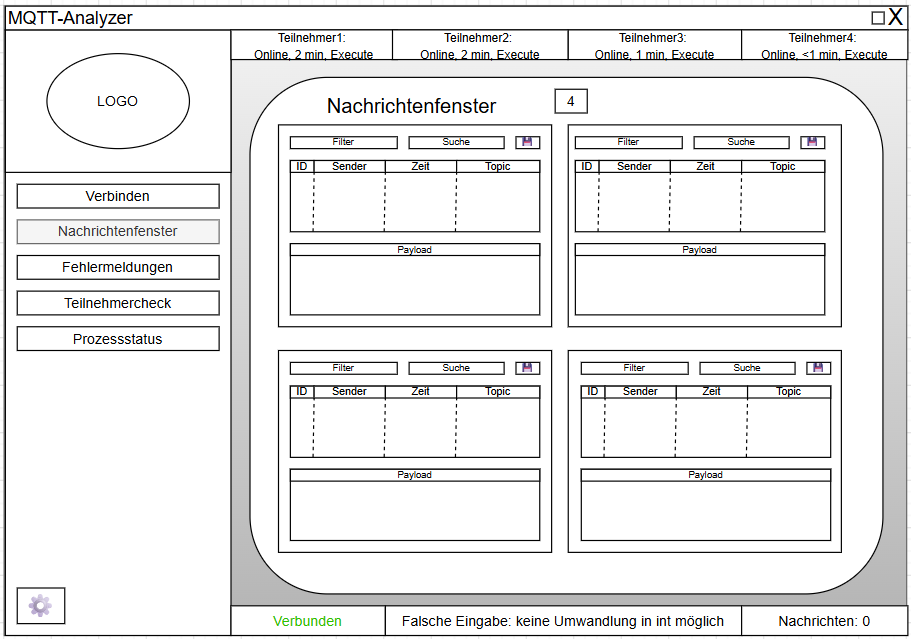
\includegraphics[width=0.8\textwidth]{images/GUIKonzept.png}
            \caption{Grundlegendes Konzept für die GUI}
            \label{fig:GUI-Konzept}
        \end{figure}

        